Los \textbf{tokens no fungibles} (\textbf{NFT}, por sus siglas en inglés) son 
activos digitales únicos que se utilizan para representar elementos digitales 
como obras de arte, videos, música, juegos, entre otros. A diferencia de las 
criptomonedas tradicionales, los NFT no son intercambiables y cada uno es 
único e irrepetible.

Los NFT se basan en la \textbf{tecnología blockchain} y utilizan contratos 
inteligentes (\textbf{smart contracts}) para garantizar la propiedad y 
autenticidad del activo digital que representan. Los contratos inteligentes 
se utilizan para definir las condiciones y términos de la transacción, y 
garantizan que solo el propietario del NFT tenga derecho a la propiedad del 
elemento digital que representa.

Los NFT se han vuelto muy populares en el mundo del arte digital, ya que 
permiten a los artistas vender sus obras de arte como activos únicos[ 
Por ejemplo, la figura \ref*{fig:opensea-nft}] y garantizar su 
autenticidad y propiedad. También se están utilizando en otros sectores como 
los videojuegos, donde se pueden utilizar para representar objetos y personajes 
únicos [Por ejemplo, la figura \ref*{fig:sorare-nft}].

\begin{figure}[htb!]
    \caption{Muestra de algunos NFT's de la collección de Moonbirds}
    \label{fig:opensea-nft}
    \centering
    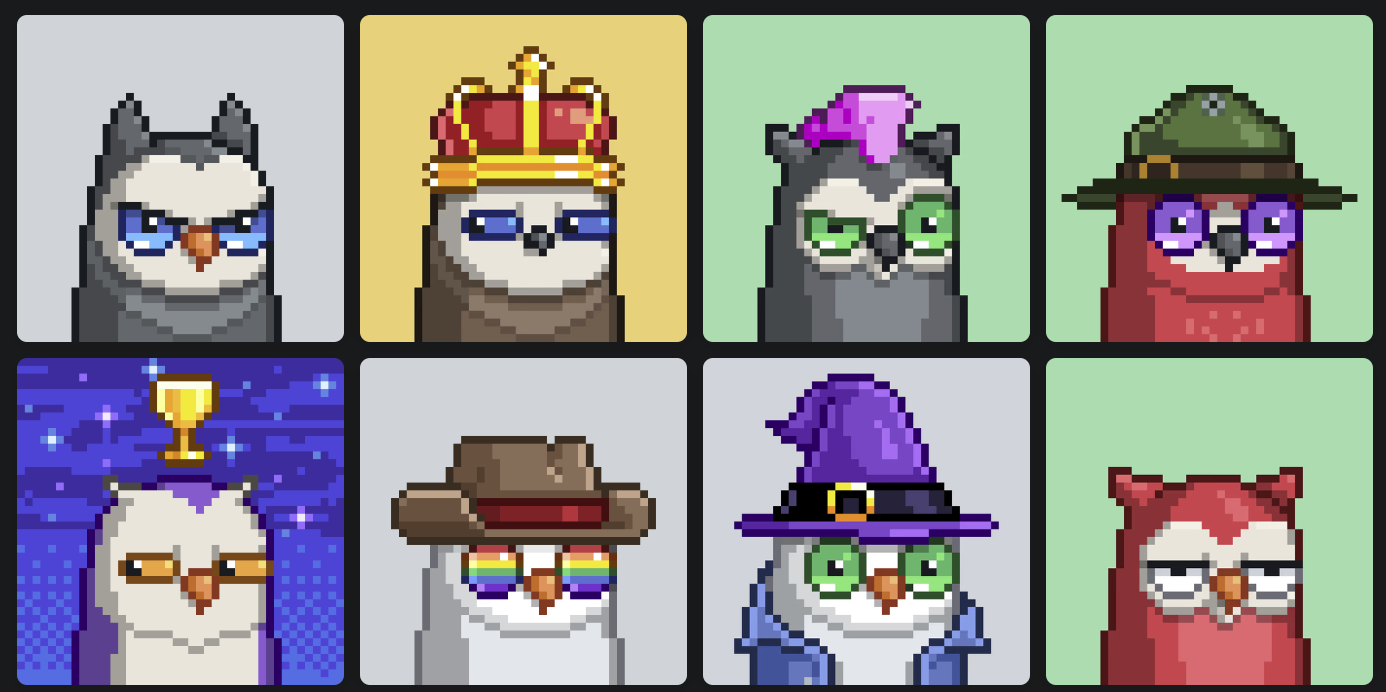
\includegraphics[scale=0.25]{./Ilustraciones/opensea-nft.png}\\
    \textbf{Fuente:} Página de OpenSea [\url{https://opensea.io}]- Collección Moonbirds
\end{figure}

\begin{figure}[htb!]
    \caption{Muestra de algunos NFT's de la Sorare}
    \label{fig:sorare-nft}
    \centering
    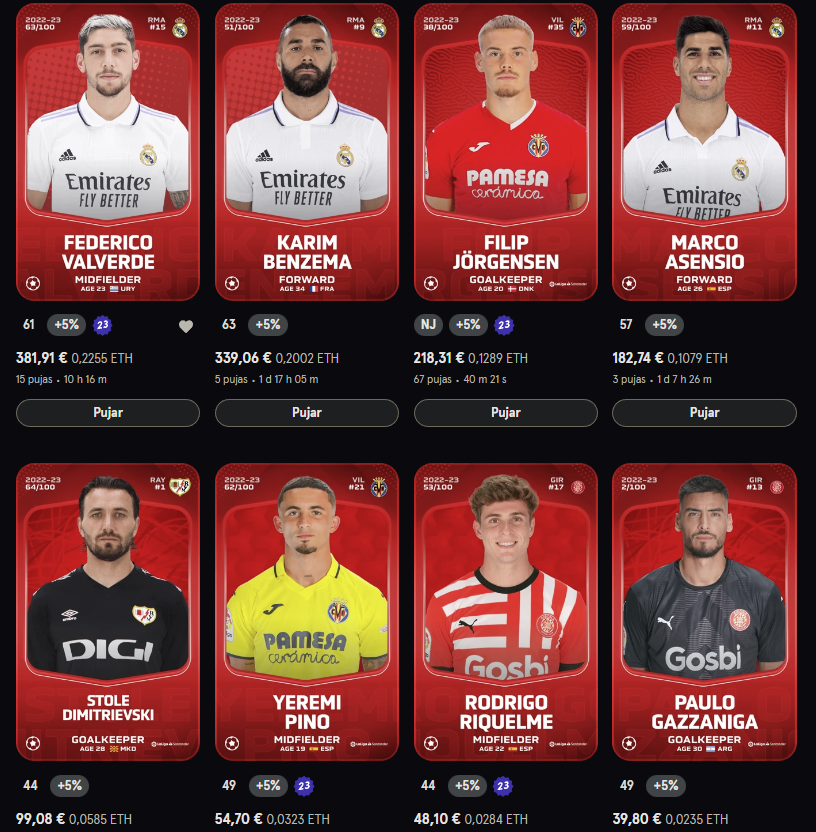
\includegraphics[scale=0.5]{./Ilustraciones/sorare-nft.png}\\
    \textbf{Fuente:} Página de Sorare [\url{https://sorare.com/}]- Sección de mercado con 
    filtros de jugador raro de la Liga Santander
\end{figure}

El valor de un NFT depende de la demanda del mercado y de la percepción del 
valor del activo digital que representa. Los NFT se pueden vender y comprar 
en plataformas especializadas y se utilizan principalmente como activos de 
inversión o de colección.

En resumen, los NFT son activos digitales únicos que se utilizan para 
representar elementos digitales como obras de arte, videos, música, juegos, 
entre otros, y se basan en la tecnología blockchain y contratos inteligentes 
para garantizar la propiedad y autenticidad del activo digital que representan. 
Los NFT se han vuelto muy populares en el mundo del arte digital y se están 
utilizando en otros sectores como los videojuegos\cite{xatakaNFT}.